\newpage
\section{429. N叉树的层序遍历}
\label{leetcode:429}

\subsection{题目}

给定一个 N 叉树,返回其节点值的层序遍历。 (即从左到右,逐层遍历)。

例如,给定一个 3叉树 :

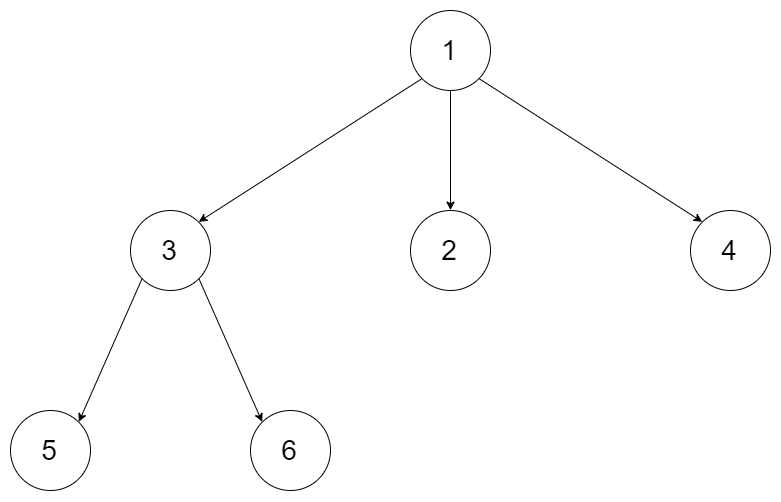
\includegraphics[width=70mm,height=50mm]{images/leetcode/leetcode_429_narytreeexample.png}

返回其层序遍历:

\begin{verbatim}
  [
    [1],
    [3,2,4],
    [5,6]
  ]
\end{verbatim}

\textbf{说明}:

\begin{itemize}
  \item 树的深度不会超过 1000。
  \item 树的节点总数不会超过 5000。
\end{itemize}

\subsection{参考题解}

\begin{verbatim}
/**
 * // Definition for a Node.
 * function Node(val,children) {
 *    this.val = val;
 *    this.children = children;
 * };
 */
/**
 * @param {Node} root
 * @return {number[][]}
 */
var levelOrder = function(root) {
  if (root === null) { return []; }
  let result = [];
  let queue = [];
  queue.push(root);
  while (queue.length > 0) {
    let currentLevel = queue;
    queue = [];
    for (let i = 0; i < currentLevel.length; i += 1) {
      let currNode = currentLevel[i];
      for (let j = 0; j < currNode.children.length; j += 1) {
        queue.push(currNode.children[j]);
      }
    }
    result.push(currentLevel.map(e => e.val));
  }
  return result;
};
\end{verbatim}
